\chapter{Entangled and Multi-Qubit Sensors}

\section{Introduction}



Quantum sensing and metrology aim to exploit quantum resources to
estimate parameters with higher precision than classical
strategies. In these notes, we introduce the theoretical foundations
of parameter estimation, from the classical Cram'er-Rao bound (CRB) in
statistics to its quantum generalization for optimally measuring
parameters encoded in quantum states. We will begin with a brief
review of classical estimation theory, defining the Fisher information
and the classical CRB. We then transition to quantum estimation
theory, defining the quantum Fisher information (QFI) and symmetric
logarithmic derivative (SLD), and derive the quantum Cram'er-Rao bound
(QCRB) for single-parameter estimation. Multi-parameter estimation
theory is discussed, including conditions under which the QCRB can be
saturated and the role of compatible measurements. We illustrate these
concepts with examples in quantum magnetometry and optical phase
estimation (e.g. GHZ states in Ramsey interferometry and N00N states),
and we examine how noise and decoherence influence QFI and estimation
precision. Optional numerical examples and pseudocode are provided to
solidify understanding. Throughout, we include important equations,
diagrams, and references to key literature.


\section{Bell, GHZ, and Squeezed States}
\section{Heisenberg Scaling and Limits}

\section{Heisenberg Limit with GHZ and Bell States}

An $N$-qubit GHZ state:
\[
\ket{\text{GHZ}} = \frac{1}{\sqrt{2}}(\ket{0}^{\otimes N} + \ket{1}^{\otimes N}),
\]
achieves QFI scaling as $N^2$, leading to the Heisenberg limit $\delta\theta \sim 1/N$.

Bell states (2-qubit entangled states) can enhance performance under
certain noise models.

\section{Limitations and Decoherence}

Entangled states are fragile; decoherence can destroy the
advantage. Under local dephasing, the QFI may decay exponentially with
$N$.




\section{Classical Estimation Theory Basics}

\label{sec:classical}



Before diving into quantum estimation, we review the classical theory
of parameter estimation. Consider a random variable $x$ drawn from a
probability distribution $p(x|\theta)$ that depends on an unknown
parameter $\theta$. The goal of estimation theory is to infer $\theta$
from observed data. An \textit{estimator} $\hat{\theta}(x)$ is any
function of the data used to estimate $\theta$. We often consider
unbiased estimators, satisfying $E[\hat{\theta}] = \theta$. The
precision of $\hat{\theta}$ is characterized by its variance
$\Var(\hat{\theta})$. The \textit{Cram'er-Rao bound} gives a
fundamental lower limit on this variance in terms of the
\textit{Fisher information}.



\subsection{Fisher Information and Cramer-Rao Bound}



The \textbf{Fisher information} (FI) measures the amount of information that an observable random variable $x$ carries about the parameter $\theta$. It is defined as

\begin{equation}

F(\theta) ;=; \mathbb{E}!\Bigg[\Big(\frac{\partial}{\partial \theta}\ln p(x|\theta)\Big)^2\Bigg] ,,

\label{eq:FI-def}

\end{equation}

where the expectation is over $x\sim p(x|\theta)$. Intuitively, $F(\theta)$ is large if the likelihood function $p(x|\theta)$ is very sensitive to changes in $\theta$. An equivalent expression is $F(\theta) = \int \frac{1}{p(x|\theta)}\left(\frac{\partial p(x|\theta)}{\partial \theta}\right)^2 dx$.



The \textbf{Cram'er-Rao bound} (CRB) states that for any unbiased estimator $\hat{\theta}$ of $\theta$, its variance is bounded by the inverse of the Fisher information:

\begin{equation}

\Var(\hat{\theta}) ;\ge; \frac{1}{F(\theta)} ,.

\label{eq:CRB-classical}

\end{equation}

In other words, the Fisher information sets a lower bound on the
estimator’s mean-squared error. The equality $\Var(\hat{\theta}) =
1/F(\theta)$ can be attained in the limit of large data
(asymptotically unbiased estimators) under regularity conditions,
e.g. by the efficient maximum likelihood estimator \cite{Kay1993}. If
we have $N$ independent and identically distributed (i.i.d.) samples
$x_1,\dots,x_N$ drawn from $p(x|\theta)$, the total Fisher information
scales linearly, $F_{\text{tot}} = N F(\theta)$, and the CRB becomes
$\Var(\hat{\theta}) \ge 1/(N F(\theta))$. This expresses the intuitive
$\frac{1}{\sqrt{N}}$ scaling of precision with number of independent
measurements (the standard quantum limit or shot-noise scaling, in
analogy with independent particles or photons).



\subsection{Multiple Parameters and Fisher Information Matrix}



The classical CRB can be generalized to the case of estimating a
vector of parameters $\vec{\theta} =
(\theta_1,\theta_2,\dots,\theta_d)$. The Fisher information becomes a
matrix $F_{ij}(\vec{\theta}) = \mathbb{E}\left[ \frac{\partial \ln
    p(x|\vec{\theta})}{\partial \theta_i}\frac{\partial \ln
    p(x|\vec{\theta})}{\partial \theta_j} \right]$,
known as the
Fisher information matrix (FIM). The multi-parameter Cram'er-Rao
inequality reads

\begin{equation}

\Cov(\hat{\vec{\theta}}) \succeq F(\vec{\theta})^{-1} ,,

\end{equation}

meaning that the covariance matrix of any unbiased estimator is at
least the inverse of the FIM (here $A \succeq B$ denotes that $A - B$
is positive semi-definite). In particular, for any unbiased estimator
of $\theta_i$, we have $\Var(\hat{\theta}i) \ge [F^{-1}]{ii}$. In the
multi-parameter case, the CRB can be saturated simultaneously for all
parameters only under certain conditions (e.g. when the likelihood has
a Gaussian form or when the estimators for different parameters
decouple) \cite{Kay1993}. In general, there can be trade-offs between
precisions of different parameters.



This classical estimation framework sets the stage. We next explore
how quantum mechanics modifies the scenario: instead of directly
sampling from $p(x|\theta)$, we now must consider probabilities
arising from measurements on a quantum state that encodes the
parameter $\theta$.



\section{Quantum Estimation Theory: Quantum Fisher Information and SLD}

\label{sec:quantum-estimation}



In quantum parameter estimation, the parameter $\theta$ is not
directly measured, but is encoded in the state of a quantum
system. Typically, one has a family of quantum states $\rho_\theta$
(density operators) that depend on $\theta$. For example, $\rho_\theta
= U_\theta \rho_0 U_\theta^\dagger$ for some initial state $\rho_0$
and a parameter-dependent unitary $U_\theta = e^{-i\theta H}$, where
$H$ is the Hamiltonian generating the parameter encoding (e.g. an
evolution Hamiltonian or a parameter-coupling observable). To estimate
$\theta$, one must perform a measurement on the quantum state and then
use a classical estimator on the measurement outcomes.



A crucial difference from the classical case is that we have the
freedom to choose what measurement to perform on the quantum
state. Different measurements (POVMs – positive operator-valued
measures) on $\rho_\theta$ will yield different outcome distributions
$p(x|\theta)$, and hence different Fisher informations. Quantum
estimation theory asks: what is the maximum achievable precision
(smallest variance) in estimating $\theta$, optimized over all
possible quantum measurements? The answer is given by the
\textit{quantum Fisher information}.



\subsection{Quantum Fisher Information (QFI)}



For a given quantum state $\rho_\theta$, and a chosen POVM measurement
with outcomes $x$, one can compute the classical FI $F(\theta)$ as in
Eq.~\eqref{eq:FI-def} from the outcome distribution $p(x|\theta) =
\Tr[\rho_\theta E_x]$ (where ${E_x}$ are the POVM elements). The
\textbf{Quantum Fisher Information} $F_Q(\theta)$ is defined as the
maximum of the Fisher information over all possible measurements
\cite{BraunsteinCaves1994}:

\begin{equation}

F_Q(\theta) ;=; \max_{{E_x}} ; F(\theta;{E_x}) ,,

\end{equation}

where $F(\theta;{E_x})$ denotes the Fisher information obtained with
measurement ${E_x}$. In other words, $F_Q$ quantifies the ultimate
precision limit encoded in the state $\rho_\theta$, irrespective of
measurement strategy (assuming one can perform the optimal
measurement).



One might expect that the optimal measurement is the one that
diagonalizes the state in a basis that is most sensitive to changes in
$\theta$. Indeed, for pure states $|\psi_\theta\rangle$, the optimal
measurement is a projective measurement in the basis
${|\psi_{\theta+\delta}\rangle - |\psi_{\theta-\delta}\rangle,
  \ldots}$ (informally, the basis that diagonalizes the derivative
$|\partial_\theta \psi_\theta\rangle$ in the two-dimensional subspace
spanned by $|\psi_\theta\rangle$ and its orthogonal component)
\cite{BraunsteinCaves1994}. For mixed states, the situation is more
complicated, but the quantum Fisher information can be computed via
the symmetric logarithmic derivative.



\subsection{Symmetric Logarithmic Derivative (SLD) and QFI Formula}



The \textbf{symmetric logarithmic derivative} $L_\theta$ is an operator defined implicitly by the equation

\begin{equation}

\frac{\partial \rho_\theta}{\partial \theta} ;=; \frac{1}{2},\big( L_\theta,\rho_\theta ;+; \rho_\theta,L_\theta \big) ,.

\label{eq:SLD-def}

\end{equation}

This equation means $L_\theta$ is the operator that, when symmetrically averaged with $\rho_\theta$, yields the derivative of the state. In general, solving for $L_\theta$ involves working in the eigenbasis of $\rho_\theta$. If $\rho_\theta$ has spectral decomposition $\rho_\theta = \sum_i \lambda_i |\psi_i(\theta)\rangle\langle \psi_i(\theta)|$ (with $\lambda_i\ge0$ and possibly depending on $\theta$), then one finds

\begin{equation}

L_\theta ;=; \sum_{i,j:;\lambda_i + \lambda_j > 0} \frac{2}{\lambda_i + \lambda_j} \langle \psi_i|\partial_\theta \rho_\theta|\psi_j \rangle ;|\psi_i\rangle\langle \psi_j| ,.

\label{eq:SLD-eigenbasis}

\end{equation}

In particular, for non-degenerate $\rho_\theta$ this can be computed by inserting the derivative of $\rho_\theta = \sum_i \lambda_i |\psi_i\rangle\langle\psi_i|$ into Eq.~\eqref{eq:SLD-def}. If $\rho_\theta$ is pure, $|\psi_\theta\rangle$, then a special case applies: $\rho_\theta = |\psi_\theta\rangle\langle\psi_\theta|$ has $\rho^2=\rho$, and one can show $L_\theta = 2(|\partial_\theta \psi_\theta\rangle\langle \psi_\theta| + \langle \psi_\theta|\partial_\theta \psi_\theta\rangle, I - \text{h.c.})$, although a more convenient formula for pure states is given below.



Once $L_\theta$ is obtained, the \textbf{quantum Fisher information} can be computed as

\begin{equation}

F_Q(\theta) ;=; \Tr!\big[\rho_\theta, L_\theta^2\big] ,.

\label{eq:QFI-def}

\end{equation}

It can be shown that indeed $F_Q(\theta)$ defined this way is the same as the supremum of classical FI over all measurements \cite{Helstrom1976, Holevo2011, BraunsteinCaves1994}. In practice, one often uses alternative formulas to compute $F_Q$ without explicitly finding $L_\theta$. One useful expression is in terms of the eigen-decomposition above:

\begin{equation}

F_Q(\theta) ;=; \sum_{i,j:; \lambda_i + \lambda_j >0} \frac{2}{\lambda_i + \lambda_j} \left|\langle \psi_i(\theta)|\partial_\theta \rho_\theta|\psi_j(\theta)\rangle\right|^2 ,.

\label{eq:QFI-eigen}

\end{equation}

For a \textit{pure state} $|\psi_\theta\rangle$, this simplifies considerably. Writing $|\partial_\theta \psi_\theta\rangle$ for the derivative with respect to $\theta$, one obtains:

\begin{equation}

F_Q(\theta) ;=; 4 \Big[, \langle \partial_\theta \psi_\theta | \partial_\theta \psi_\theta \rangle ;-; \big|\langle \psi_\theta | \partial_\theta \psi_\theta \rangle\big|^2,\Big] ,.

\label{eq:QFI-pure}

\end{equation}

This formula is analogous to the classical FI formula but for the quantum state parameter manifold. In particular, if $|\psi_\theta\rangle = e^{-i\theta H}|\psi_0\rangle$ (a unitary encoding with generator $H$ acting on the initial state $|\psi_0\rangle$), then one can show $F_Q = 4,\Var_{|\psi_0\rangle}(H)$, i.e. four times the variance of $H$ in the initial state \cite{BraunsteinCaves1994, Paris2009}. This is a useful rule of thumb: the more the state “splays out” into orthogonal directions in Hilbert space as $\theta$ changes (i.e. the bigger the variance of the generator), the higher the QFI and the better the potential precision.



\subsection{Quantum Cram'er-Rao Bound (Single Parameter)}



The quantum Fisher information sets the ultimate lower bound on the variance of any unbiased estimator $\hat{\theta}$, given the ability to perform the optimal measurement on $\rho_\theta$. The \textbf{quantum Cram'er-Rao bound} is

\begin{equation}

\Var(\hat{\theta}) ;\ge; \frac{1}{F_Q(\theta)} ,,

\label{eq:QCRB}

\end{equation}

for an unbiased estimator using the optimal measurement on the state $\rho_\theta$. This is directly analogous to the classical CRB \eqref{eq:CRB-classical}, but with $F_Q$ (which is $\ge$ any classical $F$) in place of $F$. In effect, Eq.~\eqref{eq:QCRB} sets a lower bound on the precision given the quantum state itself, before choosing a measurement. If we have $N$ copies of the state (or prepare the state $N$ times independently and perform optimal measurements on each), then the total QFI scales as $N F_Q$ and the bound becomes $\Var(\hat{\theta}) \ge 1/(N F_Q)$, matching the $\frac{1}{N}$ improvement expected for $N$ independent trials. In many quantum sensing scenarios, however, one considers using entangled states of $N$ probes or $N$ particles in a single collective state preparation to beat the $1/N$ scaling; we will discuss such cases in the examples.



It is important to note that the QCRB is in general achievable in the asymptotic limit (many repeated trials, $\theta$ estimated with effectively unbiased maximum likelihood methods) \cite{BraunsteinCaves1994, Helstrom1976}. The measurement that achieves it is typically the projective measurement in the eigenbasis of the SLD operator $L_\theta$. In other words, one should measure an observable whose eigenstates coincide with those of $L_\theta$. This measurement yields a classical Fisher information equal to the QFI, saturating the bound. In practice, the optimal measurement might depend on the (unknown) parameter $\theta$ itself, so adaptive strategies or local measurements in a neighborhood of a guessed $\theta$ may be required to reach optimal performance. Nevertheless, the QCRB provides a crucial benchmark: it tells us the very best we could possibly do, assuming the most favorable quantum measurement and estimator.



\section{Multi-Parameter Quantum Estimation}

\label{sec:multiparam}



Many quantum sensing problems involve estimating multiple parameters simultaneously (e.g. multiple phases, or a vector field with components in different directions). The extension of quantum estimation theory to the multi-parameter case is not straightforward due to potential incompatibility of optimal measurements for different parameters. Here we introduce the quantum Fisher information matrix (QFIM) and discuss conditions for the multi-parameter QCRB to be saturable.



\subsection{Quantum Fisher Information Matrix and Bound}



For a family of density matrices $\rho_{\vec{\theta}}$ depending on parameters $\vec{\theta} = (\theta_1,\theta_2,\ldots,\theta_d)$, one can define SLD operators $L_i$ for each parameter via

\begin{equation}

\partial_{\theta_i} \rho_{\vec{\theta}} ;=; \frac{1}{2}(L_i,\rho_{\vec{\theta}} + \rho_{\vec{\theta}},L_i) ,,

\end{equation}

in analogy to Eq.\eqref{eq:SLD-def}. The \textbf{quantum Fisher information matrix} (QFIM) has components given by

\begin{equation}

(F_Q){ij} ;=; \frac{1}{2}, \Tr!\Big[\rho{\vec{\theta}} (L_i L_j + L_j L_i)\Big] ,.

\label{eq:QFIM-def}

\end{equation}

Equivalently, one can write $(F_Q){ij} = \Tr[\partial{\theta_i}\rho, (G_j)]$ where $G_j$ is the symmetric operator defined by $G_j = \frac{1}{2}(L_j \rho + \rho L_j) = \partial_{\theta_j}\rho$ (i.e. $G_j$ is just the derivative of the state). In the eigenbasis form, a generalization of Eq.\eqref{eq:QFI-eigen} gives matrix elements for QFIM:

\begin{equation}

(F_Q){ij} ;=; \sum{m,n} \frac{2}{\lambda_m + \lambda_n} \Re\big[\langle \psi_m|\partial_{\theta_i}\rho|\psi_n\rangle, \langle \psi_n|\partial_{\theta_j}\rho|\psi_m\rangle\big] ,,

\end{equation}

with $\rho = \sum_m \lambda_m |\psi_m\rangle\langle \psi_m|$. For pure states, $F_Q$ is simpler: if $|\psi_{\vec{\theta}}\rangle$ is pure, then $(F_Q)_{ij} = 4,\Re[\langle \partial_i \psi | \partial_j \psi \rangle - \langle \partial_i \psi|\psi\rangle\langle\psi|\partial_j \psi\rangle]$.



The QFIM provides a matrix bound (the \textbf{quantum multi-parameter Cram'er-Rao bound}) on the covariance matrix of any unbiased multi-parameter estimator $\hat{\vec{\theta}}$:

\begin{equation}

\Cov(\hat{\vec{\theta}}) ;\succeq; F_Q(\vec{\theta})^{-1} ,.

\label{eq:QCRB-multi}

\end{equation}

This means $ \Cov(\hat{\vec{\theta}}) - F_Q^{-1}$ is positive semi-definite, and in particular $\Var(\hat{\theta}i) \ge (F_Q^{-1}){ii}$ for each component. Just as in the classical multi-parameter case, one usually cannot simultaneously saturate all components of this matrix inequality unless certain conditions hold.



\subsection{Compatible Measurements and Simultaneous Saturation}



A fundamental new feature in the quantum multi-parameter scenario is that the optimal measurements for different parameters might be incompatible. In the single-parameter case, measuring in the eigenbasis of the SLD $L_\theta$ yields the maximum Fisher information for that parameter. However, if we have multiple parameters with SLDs $L_1, L_2, \ldots$, there may not exist a single measurement that simultaneously diagonalizes all $L_i$ operators. This is only possible if the SLDs commute with each other (at least at the true value of the parameters):

\begin{equation}

[L_i, L_j] = 0 \qquad \text{for all } i,j ,.

\label{eq:SLD-comm}

\end{equation}

If this commutativity condition holds (and the eigenbases of the $\rho_{\vec{\theta}}$ do not themselves depend on $\vec{\theta}$ too strongly), then one can find a common eigenbasis of all $L_i$ and measure in that basis. In such a case, the classical Fisher information matrix for that measurement equals the QFIM, and the bound \eqref{eq:QCRB-multi} can be saturated for all parameters simultaneously \cite{Ragy2016}. Essentially, the parameters are then said to be \textit{compatible}, and there is no trade-off in their joint estimation.



If the SLDs do not commute, then there is an inherent trade-off. A measurement that is optimal for estimating $\theta_1$ will generally not be optimal for $\theta_2$, etc. No single POVM can attain the individual QFIs for all parameters at once. In these cases, one may resort to strategies like measuring different parameters in separate experimental runs, or using adaptive measurements, or more sophisticated general quantum bounds like the Holevo Cram'er-Rao bound \cite{Holevo2011} which addresses the optimal trade-off given a desired weighting of the parameter estimation errors.



An intuitive example is the simultaneous estimation of two non-commuting observables’ expectation values. If $\theta_1$ is a phase shift and $\theta_2$ is a loss parameter in an interferometer, the optimal measurement for phase (an interferometric phase measurement) is not optimal for loss (which might require photon counting), and vice versa; one cannot do both optimally at the same time because the optimal observables do not commute. The consequence is that the total estimation error has a lower bound larger than one might naively expect from independent single-parameter considerations.



Researchers have developed various approaches for handling such situations, including joint measurements with optimized positive operator-valued measures that yield good compromises, or entangling the probe with ancillary systems to allow simultaneous extraction of information about multiple parameters. However, a full exploration of multi-parameter quantum metrology is beyond our scope here (we refer the interested reader to recent reviews such as \cite{Ragy2016} for deeper discussion). In the remainder of these notes, we will mainly focus on single-parameter quantum sensing scenarios, but keep in mind that multi-parameter issues can arise in realistic sensors (for example, estimating both amplitude and phase of a field).



\section{Illustrative Examples in Quantum Sensing}

\label{sec:examples}



We now discuss several key examples of quantum parameter estimation in sensing scenarios, highlighting how the QCRB and QFI concepts are applied. We focus on two paradigmatic cases: \textbf{quantum magnetometry via Ramsey interferometry} (using entangled spin states like GHZ states), and \textbf{optical phase estimation in interferometry} (using exotic photonic states such as NOON states). These examples illustrate how quantum entanglement and quantum resources can enhance sensitivity (increase Fisher information), and we will also foreshadow how noise can impact these advantages.



\subsection{Quantum Magnetometry and Ramsey Interferometry (GHZ States)}

\label{sec:GHZ-Ramsey}



One important task in quantum metrology is measuring a weak magnetic field (or equivalently, a small frequency or phase shift accumulated due to a field) with high precision. Ramsey interferometry is a common technique in atomic clocks and magnetometers. In the simplest Ramsey scheme, a two-level atom (like a spin-$\frac{1}{2}$ or a qubit) is prepared in an equal superposition state $(|0\rangle + |1\rangle)/\sqrt{2}$ (this can be done via a $\pi/2$ pulse). The state accumulates a relative phase between $|0\rangle$ and $|1\rangle$ proportional to the energy splitting or Larmor frequency difference $\omega$ (which is proportional to the magnetic field $B$ if the two levels have a magnetic moment difference). After a time $t$, the state becomes $(|0\rangle + e^{-i\omega t}|1\rangle)/\sqrt{2}$. A second $\pi/2$ pulse is then applied, converting the phase difference into a population difference, which can be measured by checking whether the atom is in state $|0\rangle$ or $|1\rangle$. By repeating this procedure, one can estimate $\omega$ (hence $B$) from the measured outcomes. For small $\omega t$, the probability of finding $|1\rangle$ is $P_1 \approx \frac{1}{2}[1 - \sin(\omega t)]$, which has a dependence on $\omega$ that allows estimation. In this simple single-particle interferometer, the (classical) Fisher information per trial can be calculated and is proportional to $t^2$ (at small $\omega t$), giving a variance scaling $\Var(\hat{\omega}) \sim 1/t^2$. However, $t$ cannot be increased arbitrarily due to decoherence (the atom may lose phase coherence if kept too long). With $N$ independent atoms each doing Ramsey in parallel (each prepared and measured independently), the net effect is that the estimate of $\omega$ improves by $1/\sqrt{N}$ (from averaging $N$ independent samples), which is the standard quantum limit (SQL) scaling.



Quantum entanglement offers a route to surpass the SQL. A famous example is the Greenberger-Horne-Zeilinger (\textbf{GHZ}) state (also known as a cat state in this context) of $N$ two-level atoms:

\begin{equation}

|\Psi_{\text{GHZ}}\rangle ;=; \frac{1}{\sqrt{2}}\Big(|0 0 \cdots 0\rangle ;+; |1 1 \cdots 1\rangle\Big) ,,

\label{eq:GHZ-state}

\end{equation}

i.e. an equal superposition of all $N$ being in state $|0\rangle$ and all $N$ being in $|1\rangle$. This state can be prepared, for example, by entangling $N$ atoms (as has been done with trapped ions and cold atoms). If we use this state as the input to our Ramsey sequence (instead of $N$ independent superpositions), how does the phase $\omega t$ affect it? Each $|1\rangle$ picks up phase $e^{-i\omega t}$ relative to $|0\rangle$. Therefore, the $|11\cdots1\rangle$ component picks up a phase $e^{-i N \omega t}$ relative to $|00\cdots0\rangle$ (since all $N$ particles contribute). The state after free evolution is

|\Psi_{\text{GHZ}}(t)\rangle = \frac{1}{\sqrt{2}}\Big(|0\cdots0\rangle + e^{-i N \omega t} |1\cdots1\rangle\Big) \,.

Comparing to Eq.~\eqref{eq:GHZ-state}, we see the GHZ state accumulates an $N$-fold phase $N\omega t$. This means that the state is much more sensitive to the parameter $\omega$: a small change in $\omega$ produces a larger relative phase change $N\delta\omega t$. In terms of quantum Fisher information, one can calculate (using e.g. $F_Q = 4,\Var(H)$ for pure states under unitary $U=e^{-i\omega J_z t}$, where $J_z = \frac{1}{2}\sum_{k=1}^N \sigma^{(k)}_z$) that

F_Q = N^2 t^2

for the GHZ state (since the total $J_z$ for the GHZ superposition has eigenvalues $\pm \frac{N}{2}$, variance $N^2/4$). In contrast, for $N$ independent atoms each in $(|0\rangle+|1\rangle)/\sqrt{2}$, the QFI would be $N \times (1^2 t^2) = N t^2$, because each contributes $t^2$ and they add (this corresponds to the SQL). The GHZ state’s QFI is $N$ times larger, suggesting that the CRB on $\omega$ (or equivalently $B$) is $1/(N^2 t^2)$ instead of $1/(N t^2)$, an $N$-fold improvement in standard deviation (i.e. $\sim 1/N$ scaling, the \textit{Heisenberg limit}). In principle, using GHZ states can lead to Heisenberg scaling in precision with the number of particles, which is a major quantum advantage.



How is this achieved in practice? After the GHZ state accumulates the
phase, one must measure it in an appropriate basis to extract the
phase information. The optimal measurement here is effectively a
parity or collective $J_x$ measurement (a basis like
$(|0\cdots0\rangle \pm |1\cdots1\rangle)/\sqrt{2}$). If one measures
each particle individually in the ${|0\rangle,|1\rangle}$ basis, the
GHZ state’s phase cannot be discerned from a single measurement
because each single atom is random 0 or 1 with $50\%$ probability (the
entanglement means only the $N$-body correlations carry the
phase). Instead, one could perform a collective measurement (like
recombining the paths on an interferometer or via a final entangling
operation and measuring parity). In ion trap experiments, this has
been done by applying another $\pi/2$ pulse collectively to the GHZ
state to map phase to population difference, similarly to the single
atom case but now acting on the entangled state (this is the entangled
Ramsey sequence). J. Bollinger \textit{et al.} (1996)
\cite{Bollinger1996} proposed and analyzed this scheme, showing that
with GHZ states one could in principle achieve the $1/N$ phase
uncertainty.



\paragraph{Ramsey Spectroscopy with GHZ vs Unentangled Atoms:} It is instructive to compare outcomes:



With $N$ unentangled atoms: After evolution and final $\pi/2$ pulses,
each atom has probability $\approx \frac{1}{2}[1 - \sin(\omega t)]$ of
being in $|1\rangle$. If $\omega$ is small, the signal (population
difference) changes linearly with $\omega$. Repeating with $N$ atoms
yields an estimate with standard error $\delta\omega \approx
1/(\sqrt{N} t)$ (for short $t$) after one trial, which can be improved
with $M$ trials to $\approx 1/\sqrt{M N}t$.  With $N$ entangled atoms
in a GHZ: After evolution time $t$ and final recombination, the
probability to find, say, all atoms in state $|0\rangle$ vs all in
$|1\rangle$ oscillates as $\frac{1}{2}[1 - \sin(N \omega t)]$. The
collective state parity oscillates $N$ times faster with $\omega$. As
a result, a small $\omega$ causes a phase shift $N\omega t$, and the
sensitivity (slope of signal vs $\omega$) is $N$ times steeper. The
Fisher information analysis confirms $\delta\omega$ can be as low as
$1/(N t\sqrt{M})$ with $M$ repetitions, an $N$-fold gain.




Crucially, however, entanglement is not a free lunch. GHZ states are
notoriously fragile to noise, as we discuss in
Section~\ref{sec:noise}. In an ideal, noiseless scenario, GHZ states
reach the Heisenberg limit. But even small decoherence can completely
erode the $N$-fold advantage, to the point that at large $N$ the GHZ
state can perform worse than unentangled states \cite{Huelga1997}. We
will quantify this later.



Nonetheless, GHZ states and Ramsey interferometry are a cornerstone
example of quantum metrology, illustrating how entanglement can
concentrate information in collective degrees of freedom. Many
experiments have demonstrated entanglement-enhanced magnetometry, and
related states like spin-squeezed states (which are easier to prepare
and more robust than GHZ) have achieved improved clock precision in
practice. The GHZ state represents an extreme case of entanglement,
maximizing the QFI for a given $N$ (for phase estimation tasks, GHZ
states are in fact optimal in the absence of noise). The trade-off is
that GHZ provides no information if any subset of the particles is
lost or decoheres (since the state collapses or the phase becomes
random). This motivates use of other states or error-correcting
strategies in realistic sensors.



\subsection{Optical Phase Estimation: NOON States and Interferometry}



Another canonical example is optical interferometry, such as a
Mach-Zehnder or Michelson interferometer used in optical phase sensing
(e.g. gravitational wave detectors like LIGO, or fiber optical
sensors). In a Mach-Zehnder interferometer, a phase difference $\phi$
between the two arms will create an interference pattern at the
output. With classical light (coherent states or laser light at the
shot-noise limit), the phase uncertainty is limited by $\delta \phi
\sim 1/\sqrt{N_{\text{ph}}}$ where $N_{\text{ph}}$ is the number of
photons used (again a $\frac{1}{\sqrt{N}}$ scaling). Quantum optics
provides special states of light that can beat this limit. A famous
example is the \textbf{NOON state} for two modes (two arms of the
interferometer):

\begin{equation}

|\Psi_{\text{NOON}}\rangle ;=; \frac{1}{\sqrt{2}}\big(|N\rangle_a |0\rangle_b ;+; |0\rangle_a |N\rangle_b \big) ,,

\label{eq:NOON}

\end{equation}

where $|N\rangle_a$ means $N$ photons in arm $a$ and $|0\rangle_b$
means 0 in arm $b$, etc. This state is the photonic analogue of the
GHZ state: all $N$ photons are either in arm $a$ or all in arm $b$,
creating a superposition. If a phase $\phi$ is applied in arm $a$
relative to $b$, the state becomes $(|N,0\rangle + e^{-i N
  \phi}|0,N\rangle)/\sqrt{2}$, picking up a phase $N\phi$. At the
interferometer output, this leads to interference fringes in the
detection probabilities with period $2\pi/N$ (super-resolving
fringes), and an ideal phase uncertainty $\delta\phi \sim 1/N$ for
small $\phi$. The QFI of the NOON state for phase $\phi$ is $F_Q =
N^2$, again Heisenberg scaling. By contrast, a coherent state
$|\alpha\rangle$ with mean photon number $N$ has essentially $F_Q
\approx N$ (shot noise limit; more precisely, a coherent state with
$N$ photons has Poisson number distribution and achieves the standard
quantum limit). Squeezed vacuum states can reach $F_Q > N$ (giving
some improvement, which LIGO and others exploit), but states like NOON
maximize it.



The challenge with NOON states is that they are difficult to create
for large $N$, and even more sensitive to loss: if even one photon is
lost, the state collapses into an indeterminate photon-number state
that carries almost no phase information. In a lossy interferometer, a
state with a huge photon-number variance (like NOON) suffers
greatly. On the other hand, certain less extreme entangled or squeezed
states can offer a compromise of improved precision and
robustness. For instance, a \emph{twin squeezed vacuum} state or
two-mode squeezed state can provide Heisenberg-like scaling while
being more robust to loss in some regimes. Another alternative is
using Holland-Burnett state (two-mode squeezed coherent state) or Fock
states that are not maximally entangled but still provide some
advantage.



Nonetheless, conceptually, NOON states demonstrate the quantum
limit. If one could maintain them, the QCRB for $\phi$ would be
$\Var(\hat{\phi}) \ge 1/(N^2)$ (for one shot; with many shots $M$,
$1/(M N^2)$). They also illustrate multi-parameter issues: in an
interferometer with loss, one often has to estimate both $\phi$ and a
loss parameter; NOON states cannot simultaneously be optimal for both
because the best measurement for phase is not the best for loss.



\paragraph{Example: Phase Estimation with Coherent vs NOON state.} Suppose we have $N$ photons to use.



If we send a coherent state with $\bar{n}=N$ (and a vacuum in the
other input port of the interferometer), the output is a coherent
state with shot-noise-limited phase uncertainty $\delta \phi \approx
1/\sqrt{N}$ (more precisely, the FI for phase is $N$ for a coherent
state detected at the dark port).  If we send a NOON state of $N$
photons, and measure an appropriate observable (e.g. parity at one
output port or perform quantum interference counts), one can achieve
$\delta \phi \approx 1/N$. However, if one of those $N$ photons is
lost, the effective state collapses to something like a mixture that
gives much less information. In fact, it can be shown that with a loss
probability $p$ per photon, the variance of phase estimation with a
NOON state scales poorly for large $N$ (there is an optimal $N$ beyond
which adding more photons worsens the precision due to increased
chance of losing at least one photon). By contrast, a coherent state’s
precision degrades more gracefully with loss.




This highlights a general point: while $F_Q$ is an important figure of
merit, it assumes an optimal, often entangled probe state. In
realistic conditions (noise, loss), the effective QFI might scale
differently. Often, for small $N$ entanglement helps, but as $N$
grows, noise can impose an effective limit (see next section).



\section{Effects of Noise and Decoherence on QFI and Precision}

\label{sec:noise}



In practice, quantum sensors are subject to various noise and
decoherence processes. These could include spontaneous emission,
dephasing, photon loss, thermal noise, imperfect controls, etc. Such
processes typically reduce the quantum Fisher information, sometimes
drastically. Understanding how $F_Q$ behaves under noise is key to
determining whether a quantum advantage survives in a given scenario.



We will discuss qualitatively how noise impacts some of our earlier
examples, and present a small quantitative analysis for GHZ states
under decoherence. A general observation is that \emph{entangled
states tend to be more fragile to noise than unentangled ones}. As a
result, the Heisenberg scaling often does not hold up indefinitely
with increasing $N$ in the presence of decoherence; instead, one often
reverts to shot-noise scaling for sufficiently large $N$ (or at best a
modest constant-factor improvement over the best classical strategy).



\subsection{Noise in Ramsey Magnetometry (GHZ with Dephasing/Decay)}



Consider the atomic GHZ Ramsey example in Section~\ref{sec:GHZ-Ramsey}. In a real atomic clock or magnetometer, each atom might undergo spontaneous emission (if $|1\rangle$ is an excited state) or dephasing due to magnetic field fluctuations, etc. Huelga \textit{et al.} (1997) \cite{Huelga1997} analyzed a model where each of $N$ two-level atoms has a probability of spontaneous emission during the Ramsey interrogation time $t$. Spontaneous emission is an example of decoherence (it not only randomizes phase but can flip the state out of the two-level subspace). The result was striking: the GHZ state’s precision advantage is highly susceptible to this noise. In fact, they found that the optimal Ramsey interrogation time for a GHZ state shrinks as $N$ grows (because waiting longer allows more chance for an atom to decay, which ruins the GHZ state), and the net gain over $N$ unentangled atoms is lost for large $N$. The best that can be achieved in that model was a constant-factor improvement (like  constant $\approx \sqrt{2}$ advantage) but \emph{not} a scaling improvement.



To illustrate the effect of dephasing noise, let’s consider a simpler model: pure dephasing of each qubit (no energy relaxation, just phase damping). Suppose each atom accumulates a phase $\omega t$ as before, but in addition, each has a coherence factor $e^{-\Gamma t}$ due to some stochastic phase noise (with rate $\Gamma$). This transforms the pure state into a mixed state. For a \emph{single qubit} initially $(|0\rangle+|1\rangle)/\sqrt{2}$, after time $t$ the off-diagonal element of its density matrix decays as $e^{-\Gamma t}$:

\rho_1(t) = \frac{1}{2}\begin{pmatrix}1 & e^{-\Gamma t} e^{-i \omega t} \\ e^{-\Gamma t} e^{i \omega t} & 1\end{pmatrix} \,.

One can compute the QFI of this dephased single-qubit state for the parameter $\omega$. Using Eq.~\eqref{eq:QFI-eigen} or the formula for qubit states, one finds

F_{Q, \text{single}}(\omega) = t^2 e^{-2\Gamma t} \,.

At short times (small $\Gamma t$), this is approximately $t^2$ as expected (since initially it’s like no decoherence); at long times, $F_Q$ decays as the coherence is lost.



Now, for $N$ independent atoms (unentangled), each contributes $t^2 e^{-2\Gamma t}$, so

F_{Q,\text{unentangled}} = N\, t^2 e^{-2\Gamma t} \,.

This peaks at some optimal time $t_{\text{opt}}$ when $dF_Q/dt = 0$. Maximizing, one finds $t_{\text{opt}} = 1/\Gamma$ (for unentangled, roughly when $e^{-2\Gamma t}$ decays to $1/2$). The maximum QFI is $F_Q^{\max} \approx N/(2\Gamma^2 e)$ (the exact value isn’t as important; the scaling is $O(N)$, as expected).



For the $N$-qubit GHZ state under independent dephasing on each qubit,
the off-diagonal of the $N$-qubit density matrix decays as $e^{-N
  \Gamma t}$. This is because all $N$ qubits need to maintain
coherence; if any one decoheres, the GHZ superposition coherence is
lost. The state becomes (at time $t$):

\rho_{\text{GHZ}}(t) = \frac{1}{2}\Big(|0\cdots0\rangle\langle 0\cdots0| + |1\cdots1\rangle\langle 1\cdots1| + e^{-N\Gamma t} e^{-i N \omega t}|0\cdots0\rangle\langle 1\cdots1| + \text{h.c.}\Big) .

The QFI for this mixed state can be calculated (we did so numerically for small $N$ earlier). The result is

F_{Q,\text{GHZ}}(\omega) = N^2 t^2 e^{-2 N \Gamma t} \,.

This formula holds at least for the dephasing channel model and small $\omega t$. We can see the dramatic difference: although at very short times $F_Q$ grows as $N^2 t^2$, the decoherence factor is $e^{-2 N \Gamma t}$, which decays much faster with $t$ for large $N$.



What is the optimal interrogation time $t_{\text{opt}}$ for the GHZ
state? Setting derivative zero yields $t_{\text{opt}} = \frac{1}{N
  \Gamma}$ (so the larger $N$, the shorter time you should use the
entangled state before measuring, to avoid decoherence). At that
optimal time, the QFI is

F_Q^{\max,\text{GHZ}} \approx \frac{N^2}{(e^2 (N\Gamma)^2)} =
\frac{1}{e^2} \frac{N^2}{N^2 \Gamma^2} = \frac{1}{e^2 \Gamma^2} \,.

Notably, the $N$ dependence canceled out! The maximum $F_Q$ achievable
with GHZ in this dephasing model is actually independent of $N$ (aside
from the $1/e^2$ factor). This means the best possible precision (for
given noise strength $\Gamma$) does not improve with more particles
entangled—the Heisenberg scaling is completely lost. In fact, the
unentangled strategy achieved a maximum $F_Q \propto N$, which for
large $N$ will exceed the GHZ’s maximum which is constant. Thus beyond
a certain $N$, using more particles entangled is
counterproductive. There will be a crossing point where $N$
unentangled outperforms GHZ. This is precisely what Huelga \textit{et
  al.} found in the spontaneous emission case \cite{Huelga1997}: at $N
\approx \Gamma t$ etc., eventually standard Ramsey is better.



\begin{figure}[tb]

\centering

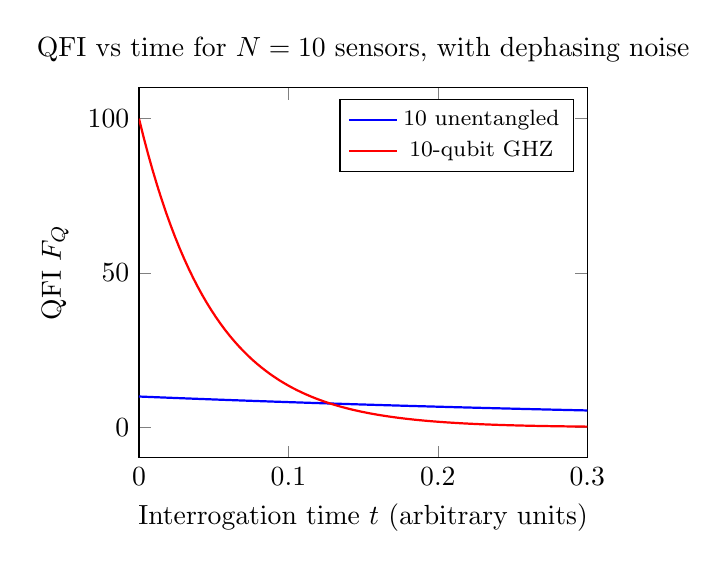
\begin{tikzpicture}

\begin{axis}[width=0.6\textwidth, xlabel={Interrogation time $t$ (arbitrary units)}, ylabel={QFI $F_Q$}, xmin=0, xmax=0.3, legend pos=north east, legend style={font=\footnotesize}, title={QFI vs time for $N=10$ sensors, with dephasing noise}, ylabel style={align=center}]

\addplot[domain=0:0.3, samples=100, thick, blue] {10 * exp(-2 * x)};

\addlegendentry{10 unentangled}

\addplot[domain=0:0.3, samples=100, thick, red] {100 * exp(-20 * x)};

\addlegendentry{10-qubit GHZ}

\end{axis}

\end{tikzpicture}

\caption{Quantum Fisher information as a function of interrogation time $t$ for estimating a phase (or frequency) with $N=10$ two-level systems under dephasing noise (rate $\Gamma=1$ unit). \textcolor{blue}{Blue curve}: $N$ unentangled atoms (each contributes $e^{-2\Gamma t}t^2$ so total $F_Q = 10 t^2 e^{-2t}$ up to units). \textcolor{red}{Red curve}: $N$-atom GHZ state ($F_Q = 100 t^2 e^{-20 t}$). At very short times, the GHZ has higher $F_Q$ (steeper initial rise), but it reaches a peak and then decays much faster. The optimum for GHZ is at a shorter $t$ than for unentangled, and yields here a slightly smaller maximum $F_Q$. In this noise regime, entanglement does not offer a long-term advantage, highlighting the fragility of GHZ states to decoherence.}

\label{fig:GHZ-dephasing}

\end{figure}



Figure \ref{fig:GHZ-dephasing} illustrates this comparison for $N=10$
and $\Gamma=1$ (in arbitrary units). We see that initially the GHZ
curve (red) surpasses the unentangled (blue), but then it drops
sharply. The unentangled $F_Q$ decays more slowly and eventually is
higher for larger $t$. Depending on what interrogation time is used,
one or the other performs better. If one optimizes $t$, the
unentangled scheme achieves a better maximum in this example.



The conclusion is that in presence of uncorrelated decoherence, the
achievable precision often obeys an \textit{effective shot-noise
  limit} even with entanglement \cite{Demkowicz2012}. More entangled
probes do not indefinitely improve the scaling; instead, there is
typically a crossover point beyond which adding more particles (or
photons) while keeping them all entangled hurts the precision due to
noise. For moderate $N$, one may still get some improvement by
entanglement, but the advantage is polynomially or even exponentially
curtailed. Various strategies to combat this involve using partially
entangled states (like spin-squeezed states which achieve $F_Q \propto
N^{\alpha}$ with $\alpha<2$ but are more robust), or employing quantum
error correction during sensing \cite{Dur2014} to actively correct for
decoherence and restore Heisenberg scaling (at the cost of overhead).



\subsection{Decoherence in Optical Interferometry}



A similar story occurs in optical interferometry with loss. If each
photon has probability $\eta$ to survive the interferometer
(transmittance $\eta$, loss $1-\eta$), then for large $N$ photons the
chance that all $N$ survive (which is roughly $\eta^N$) becomes very
small. A NOON state’s useful component is precisely the component
where all $N$ are intact; any loss collapses it. Thus the effective
Fisher information of a NOON state with loss plummets for large
$N$. It has been shown \cite{Demkowicz2012} that for any fixed loss
rate (e.g. each photon has $95\%$ survival), the asymptotic scaling of
any quantum scheme’s precision is at best shot-noise scaling; one can
at most gain a constant factor improvement (the so-called
\emph{Heisenberg limit is elusive} under noise). In practice, for
moderate $N$ (say up to 10 or 20 photons), one could see an advantage,
but not unbounded with $N$. On the other hand, if loss can be reduced
with $N$ or if certain error-correcting codes are used, one might
circumvent this.



In summary, noise and decoherence tend to reduce the quantum Fisher
information. The QCRB with noise may not scale as favorably with $N$
as the noiseless theory would suggest. Nonetheless, the QFI remains a
powerful tool: one can include the noise process in the quantum state
$\rho_\theta$ (by solving the master equation or Kraus maps for
$\rho_\theta$ with noise) and then compute $F_Q$ to know the best
possible precision in that noisy scenario. This can guide the design
of quantum sensors: for example, one might find that for a given $N$,
a certain partially entangled state has a higher $F_Q$ under noise
than the GHZ state does. Or one might find the optimal $N$ or optimal
time to use in an experiment to maximize the information.



\section{Numerical Example: Simulation of QFI Under Noise}

\label{sec:numerics}



As an optional illustration, we can simulate the quantum Fisher
information for a simple system and see the impact of noise
numerically. Consider a single qubit (spin-$\frac{1}{2}$) used to
estimate a rotation angle $\theta$. The qubit starts in state
$|+\rangle = (|0\rangle+|1\rangle)/\sqrt{2}$ (an eigenstate of
$\sigma_x$) at $\theta=0$. The parameter is encoded by a unitary
$U(\theta) = e^{-i \theta \sigma_z/2}$ (rotation about $z$-axis by
angle $\theta$). If there is no noise, the state is
$|\psi(\theta)\rangle = \frac{1}{\sqrt{2}}(|0\rangle +
e^{-i\theta}|1\rangle)$, which is exactly the Ramsey scenario we
described. The QFI for $\theta$ in this pure state can be calculated
from Eq.~\eqref{eq:QFI-pure}, or using the variance picture: here the
generator is $H=\sigma_z/2$ with variance $1/4$ in the $|+\rangle$
state, so $F_Q = 4 \times \frac{1}{4} = 1$. Indeed, one finds $F_Q =
1$ for all $\theta$; hence $\Var(\hat{\theta}) \ge 1$ (in radians$^2$)
for one shot, meaning the smallest uncertainty (one standard
deviation) is $1$ rad, which makes sense given a single qubit gives a
binary outcome at best (with many repeats $\sim \frac{1}{\sqrt{M}}$
improvement).



Now, if the qubit suffers dephasing with decoherence factor $c =
e^{-\Gamma t}$ (here $t$ would correspond to $\theta$ if $\theta$
accumulates over time $t$ linearly, but let’s treat $\theta$ as the
small parameter we estimate), the state becomes $\rho(\theta) =
\frac{1}{2}\begin{pmatrix}1 & c e^{-i\theta} \ c e^{i\theta} &
  1\end{pmatrix}$. The QFI we derived earlier for this state is $F_Q =
  c^2$ (assuming $\theta$ small or general $\theta$ since the QFI for
  phase is independent of the phase value). If $c=0.8$ for example,
  $F_Q = 0.64$. This means the best one can do is now
  $\Var(\hat{\theta}) \ge 1/0.64 \approx 1.56$ rad$^2$ per shot, a
  larger uncertainty than without dephasing. As $c \to 0$ (complete
  dephasing), $F_Q \to 0$ and you cannot estimate $\theta$ at all
  (indeed the state becomes completely mixed, which contains no
  information about $\theta$).



For a quick numerical simulation, one could randomly sample
measurement outcomes from an optimal measurement and verify the CR
bound. For brevity, we will skip a full Monte Carlo simulation here
and instead outline pseudocode:



\begin{verbatim}





Pseudocode for computing Quantum Fisher Information via diagonalization:





Define rho(theta) as a function giving the density matrix at parameter theta.

Compute drho_dtheta = derivative of rho at theta (analytically or by small delta).

Find eigenvalues {λ_i} and eigenvectors {|ψ_i>} of rho.

Compute QFI = sum_{i,j} (2/(λ_i+λ_j)) * |<ψ_i| drho_dtheta |ψ_j>|^2, summing only where λ_i+λ_j>0.

\end{verbatim}



Using this algorithm on the single-qubit example above yields $F_Q =
e^{-2\Gamma t}$ as derived. One can similarly plug in the $N$-qubit
GHZ state density matrix with dephasing and confirm $F_Q = N^2
e^{-2N\Gamma t}$.



In practice, one might use a quantum software library (like QuTiP in
Python or Julia’s QuantumOptics) to define the Lindblad dynamics,
obtain $\rho(\theta)$, and then compute QFI. For large systems, direct
diagonalization is expensive, and there are more efficient methods to
compute $F_Q$ (especially for one-parameter unitary families, where
formulas like $F_Q = 4 , \text{Var}(H)$ for pure states or a similar
Purity-based formula for mixed states can be used).



The key takeaway from numerical explorations is that $F_Q$ can be
computed for any given model, and it provides a benchmark for the best
possible precision. One can then design measurements to approach that
(often maximum likelihood estimation combined with the optimal POVM
asymptotically approaches the bound).



\section{Conclusion}



In these notes, we have provided a detailed overview of the quantum
Cram'er-Rao bound in the context of quantum sensing, guiding the
reader from classical estimation theory to quantum Fisher information
and its applications. The classical Fisher information and CRB set the
stage by showing how the variance of an estimator is bounded by the
inverse of information in data. Quantum estimation theory extends
these ideas by considering the optimization over measurements and
introducing the QFI and SLD formalism. We derived the QCRB for single
parameters, which establishes the ultimate precision limit given a
quantum state. We also discussed multi-parameter estimation,
emphasizing how the lack of commutativity of optimal measurements for
different parameters can prevent simultaneous saturation of the bound,
a peculiarly quantum phenomenon with no classical analog.



Through examples like entangled atomic GHZ states in Ramsey
interferometry and photonic NOON states in Mach-Zehnder
interferometers, we illustrated both the promise of quantum metrology
(Heisenberg scaling sensitivities and improved precision) and the
practical challenges (fragility to noise and decoherence). We saw that
while entanglement can, in principle, offer quadratic improvements in
Fisher information, in practice noise tends to limit those gains. For
instance, independent dephasing or loss can reduce the advantage of
GHZ/NOON states to the point that simpler unentangled or moderately
entangled states are preferable. These considerations underscore a key
lesson: one must always consider the full picture including noise when
predicting the performance of a quantum sensor. The QFI framework
fortunately allows one to include noise by using the quantum channel
acting on the state $\rho_\theta$ and computing $F_Q$ for the
resulting mixed state.



Finally, we provided optional numerical examples and pseudocode to
demonstrate how one might calculate QFI and verify these theoretical
results. The quantum Cram'er-Rao bound is not merely a abstract bound;
it is a practical tool that has guided the development of quantum
technologies like atomic clocks, magnetometers, and optical
interferometers. As research progresses, new techniques (such as
error-corrected metrology, adaptive measurements, and multi-parameter
estimation strategies) will further bridge the gap between these
theoretical limits and achievable precision in the laboratory. We hope
these notes serve as a solid foundation for understanding and applying
the QCRB in your own research.



